\subsection{Boot Sequence}
\begin{frame}
  \frametitle{Bootloaders}
  \begin{itemize}
  \item The bootloader is a piece of code responsible for
    \begin{itemize}
    \item Basic hardware initialization
    \item Loading of an application binary, usually an operating
      system kernel, from flash storage, from the network, or from
      another type of non-volatile storage.
    \item Possibly decompression of the application binary
    \item Execution of the application
    \end{itemize}
  \item Besides these basic functions, most bootloaders provide a
    shell with various commands implementing different operations.
    \begin{itemize}
    \item Loading of data from storage or network, memory inspection,
      hardware diagnostics and testing, etc.
    \end{itemize}
  \end{itemize}
\end{frame}

\begin{frame}
  \frametitle{Bootloaders on BIOS-based x86 (1)}
  \begin{columns}
    \column{0.8\textwidth}
    \begin{itemize}
    \item The x86 processors are typically bundled on a board with a
      non-volatile memory containing a program, the BIOS.
    \item On old BIOS-based x86 platforms: the BIOS is responsible for
      basic hardware initialization and loading of a very small piece
      of code from non-volatile storage.
    \item This piece of code is typically a 1st stage bootloader,
      which will load the full bootloader itself.
    \item It typically understands filesystem formats so that the
      kernel file can be loaded directly from a normal filesystem.
    \item This sequence is different for modern EFI-based systems.
    \end{itemize}
    \column{0.2\textwidth}
    \includegraphics[height=0.8\textheight]{slides/sysdev-bootloaders-sequence/x86-bootloader-sequence.pdf}
  \end{columns}
\end{frame}

\begin{frame}
  \frametitle{Bootloaders on x86 (2)}
  \begin{itemize}
  \item GRUB, Grand Unified Bootloader, the most powerful one.\\
    \url{https://www.gnu.org/software/grub/}
    \begin{itemize}
    \item Can read many filesystem formats to load the kernel image
      and the configuration, provides a powerful shell with various
      commands, can load kernel images over the network, etc.
    \item See our dedicated presentation for details:\\
      \url{https://bootlin.com/doc/legacy/grub/}
    \end{itemize}
  \item Syslinux, for network and removable media booting (USB key, CD-ROM)\\
    \small\url{https://kernel.org/pub/linux/utils/boot/syslinux/}\normalsize
  \end{itemize}
\end{frame}

\begin{frame}
  \frametitle{Booting on embedded CPUs: case 1}
  \begin{columns}
    \column{0.8\textwidth}
    \begin{itemize}
    \item When powered, the CPU starts executing code at a fixed address
    \item There is no other booting mechanism provided by the CPU
    \item The hardware design must ensure that a NOR flash chip is
      wired so that it is accessible at the address at which the CPU
      starts executing instructions
    \item The first stage bootloader must be programmed at this
      address in the NOR
    \item NOR is mandatory, because it allows random access, which
      NAND doesn't allow
    \item {\bf Not very common anymore} (unpractical, and requires NOR
      flash)
    \end{itemize}
    \column{0.2\textwidth}
    \includegraphics[width=\textwidth]{slides/sysdev-bootloaders-sequence/booting-from-nor.pdf}
  \end{columns}
\end{frame}

\begin{frame}
  \frametitle{Booting on embedded CPUs: case 2}
  \begin{itemize}
  \item The CPU has an integrated boot code in ROM
    \begin{itemize}
    \item BootROM on AT91 CPUs, “ROM code” on OMAP, etc.
    \item Exact details are CPU-dependent
    \end{itemize}
  \item This boot code is able to load a first stage bootloader from a
    storage device into an internal SRAM (DRAM not initialized yet)
    \begin{itemize}
    \item Storage device can typically be: MMC, NAND, SPI flash, UART
          (transmitting data over the serial line), etc.
    \end{itemize}
  \item The first stage bootloader is
    \begin{itemize}
    \item Limited in size due to hardware constraints (SRAM size)
    \item Provided either by U-Boot (called {\em Secondary Program Loader
          - SPL}), or by the CPU vendor (usefully open-source).
    \end{itemize}
  \item This first stage bootloader must initialize DRAM and other
    hardware devices and load a second stage bootloader into RAM
  \end{itemize}
\end{frame}

\begin{frame}
  \frametitle{Booting on Microchip ARM SAMA5D3}
  \begin{columns}
    \column{0.3\textwidth}
    \includegraphics[height=0.8\textheight]{slides/sysdev-bootloaders-sequence/at91-boot.pdf}
    \column{0.7\textwidth}
    \footnotesize
    \begin{itemize}
    \item {\bf RomBoot}: tries to find a valid bootstrap image from
      various storage sources, and load it into SRAM (DRAM not
      initialized yet). Size limited to 64 KB. No user interaction
      possible in standard boot mode.
    \item {\bf U-Boot SPL}: runs from SRAM. Initializes the DRAM,
      the NAND or SPI controller, and loads the secondary bootloader
      into RAM and starts it. No user interaction possible.
    \item {\bf U-Boot}: runs from RAM. Initializes some other hardware
      devices (network, USB, etc.).  Loads the kernel image from
      storage or network to RAM and starts it. Shell with commands
      provided.
    \item {\bf Linux Kernel}: runs from RAM. Takes over the system
      completely (the bootloader no longer exists).
    \end{itemize}
    Note: same process on other Microchip AT91 SoCs, but the
    SRAM size is smaller on the older ones.
  \end{columns}
\end{frame}

\begin{frame}
  \frametitle{Booting on Marvell SoCs}
  \begin{columns}
    \column{0.3\textwidth}
    \includegraphics[width=\textwidth]{slides/sysdev-bootloaders-sequence/marvell-boot.pdf}
    \column{0.7\textwidth}
    \footnotesize
    \begin{itemize}
    \item {\bf ROM Code}: tries to find a valid bootstrap image from
      various storage sources, and load it into RAM. The RAM
      configuration is described in a CPU-specific header, prepended
      to the bootloader image.
    \item {\bf U-Boot}: runs from RAM. Initializes some other hardware
      devices (network, USB, etc.).  Loads the kernel image from
      storage or network to RAM and starts it. Shell with commands
      provided. File called \code{u-boot.kwb}.
    \item {\bf Linux Kernel}: runs from RAM. Takes over the system
      completely (bootloaders no longer exists).
    \end{itemize}
  \end{columns}
\end{frame}

\begin{frame}
  \frametitle{Generic bootloaders for embedded CPUs}
  \begin{columns}
  \column{0.6\textwidth}
  \small
  There are several open-source generic bootloaders.\\
  Here are the most popular ones:
  \begin{itemize}
  \item {\bf U-Boot}, the universal bootloader by Denx
      \begin{itemize}
        \item The most used on ARM, also used on PPC, MIPS, x86, m68k, RISC-V, etc.
        \item The de-facto standard nowadays. We will study it in detail.
         \item \url{https://www.denx.de/wiki/U-Boot}
      \end{itemize}
  \item {\bf Barebox}, an architecture-neutral bootloader created by Pengutronix.
      \begin{itemize}
        \item It doesn't have as much hardware support as U-Boot yet.
	\item U-Boot has improved quite a lot thanks to this competitor.
        \item \url{https://www.barebox.org}
      \end{itemize}
  \end{itemize}
  \column{0.4\textwidth}
    \vspace{2cm}
    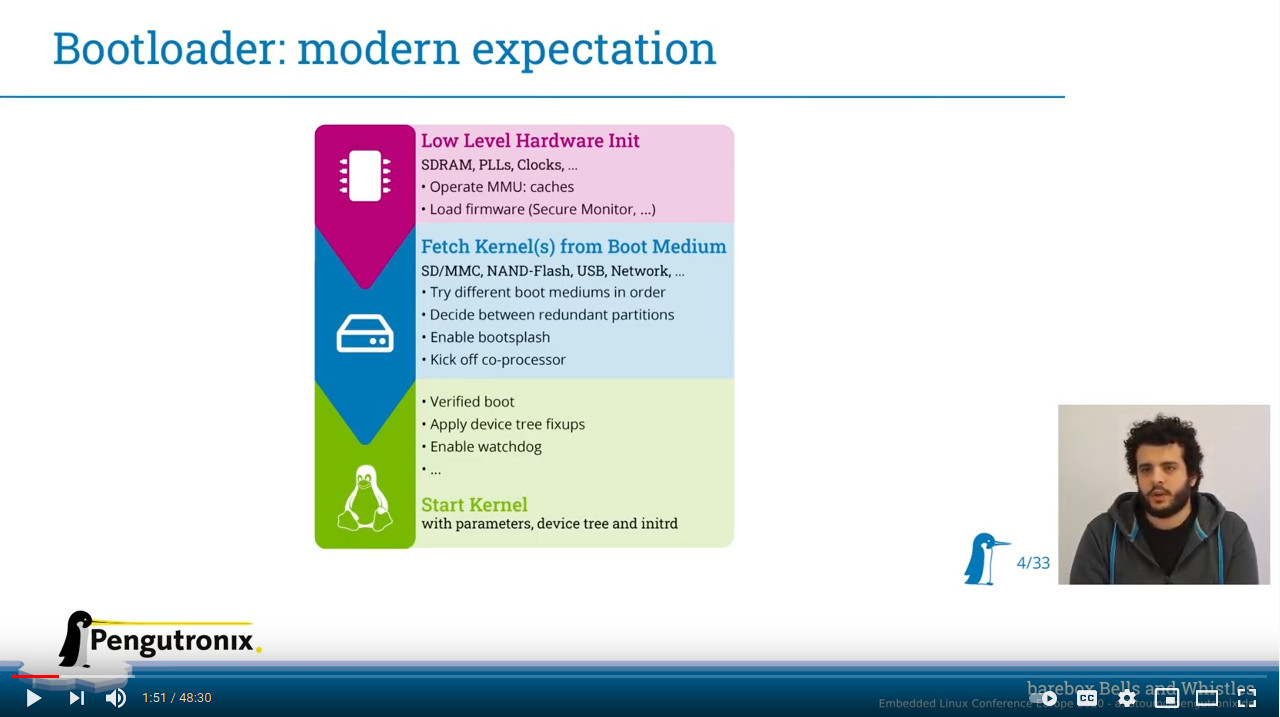
\includegraphics[width=\textwidth]{slides/sysdev-bootloaders-sequence/barebox-video.jpg}\\
    \vspace{0.3cm}
    \tiny See the nice introduction to Barebox\\
	  from Ahmad Fatoum at ELCE 2020:\\
          Video: \url{https://youtu.be/Oj7lKbFtyM0}\\
	  Slides: \url{https://elinux.org/images/9/9d/Barebox-bells-n-whistles.pdf}
  \end{columns}
\end{frame}
